\chapter{Introduction}

The discovery of single-atomic-layer graphene in 2004
inspired a new generation of research on two-dimensional semiconductors
\cite{Novoselov666}.
These 2D materials display extraordinary properties not present in the bulk.
Graphene boasts high electron mobility and exceptional strength.
Single-layer transition metal group-VI dichalcogenides (TMDs)
exhibit spin-coupled optoelectronic properties
and a new valley degree of freedom.
Monolayers are inherently flexible and transparent,
and future devices fabricated from 2D layers promise
novel applications, reduced size, and lower power requirements.

A relatively new field, breakthroughs in spintronics
have already impacted the tech industry.
In 2007, Albert Fert and Peter Grünberg were awarded
the Nobel prize in Physics for the discovery of
Giant magnetoresistance (GMR)
which found wide application in computer storage technology
\cite{PhysRevB.39.4828}.
The potential applications of 2D materials for
building new spintronic devices is equally exciting.
Such devices would encode signals in spin current
as opposed to electric current.

Building a dynamic spin transport device using a
spin degenerate material like graphene
relies on some external means to polarize the spin.
Typically, electrons are forced though a ferromagnetic contact
which polarizes the spin along a single axis.
Any viable material must be a good conductor of spin current.
As spin polarized electrons travel through a conducting channel,
internal scattering events which flip spin tend to randomize the signal.
The spin lifetime is the characteristic timescale
over which this signal will survive,
and thus it determines the length scale for a realistic device.
Finding a material with suitably long spin lifetimes
is critical for realizing any spin transport device.
While theoretical predictions for graphene suggest microsecond lifetimes,
experimental measurements report lifetimes six orders of magnitude less.

\Cref{s:spin-lifetime} of this thesis
concerns the discrepancy
between the theoretically predicted spin lifetimes in graphene
and the significantly longer experimentally measured ones.
We present an analytical solution to the drift-diffusion equation
modeling a canonical nonlocal spin value experiment which
includes the effects of the ferromagnetic contacts.
The device, shown in \cref{fig:spin-device},
is subject to a varying magnetic field,
and the resulting Hanle curve generated by measuring the spin signal
is used to extract the effective spin lifetime.
Using real data, we then analyze the reliability of fitting this model
over critical parameter regimes, particularly in the case of large lifetimes.

\begin{figure}[b]
  \centering
  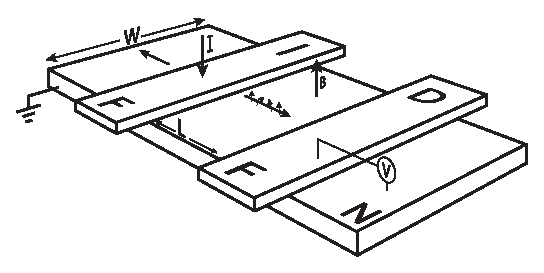
\includegraphics[width=\textwidth]{figures/device}
  \caption{%
    Isometric representation of a nonlocal spin valve in a magnetic field.
    Current is injected into the semiconductor
    through the left ferromagnetic contact.
    The strength of the diffusive spin signal is measured as a voltage
    at the right ferromagnetic contact.
  }\label{fig:spin-device}
\end{figure}

Another excellent candidate for spintronic devices,
TMDs are materials with strong spin-orbit coupling that break spin degeneracy
and provide an intrinsic means to control the spin signal.
In particular, TMDs show a strong coupling
between polarized light and their valley degree of freedom.
Since each band is spin-split, controlled optical excitations
may selectively activate carriers of a single valley and spin population.
Additionally, each valley has opposite Berry curvature, so
electrons in different valleys drift in opposite directions transverse
to an applied in-plane electric field.

\Cref{s:dichalcogenides} of this thesis
characterizes the possible superconducting phases for monolayer TMDs
in a regime where the spin and valley degrees of freedom are locked.
We consider phases arising from proximity to a normal superconductor
or effective attractive electron-electron interactions.
The valley selective optical excitation rules
and topological character are reproduced
in the context of the superconducting state.

\begin{figure}
  \centering
  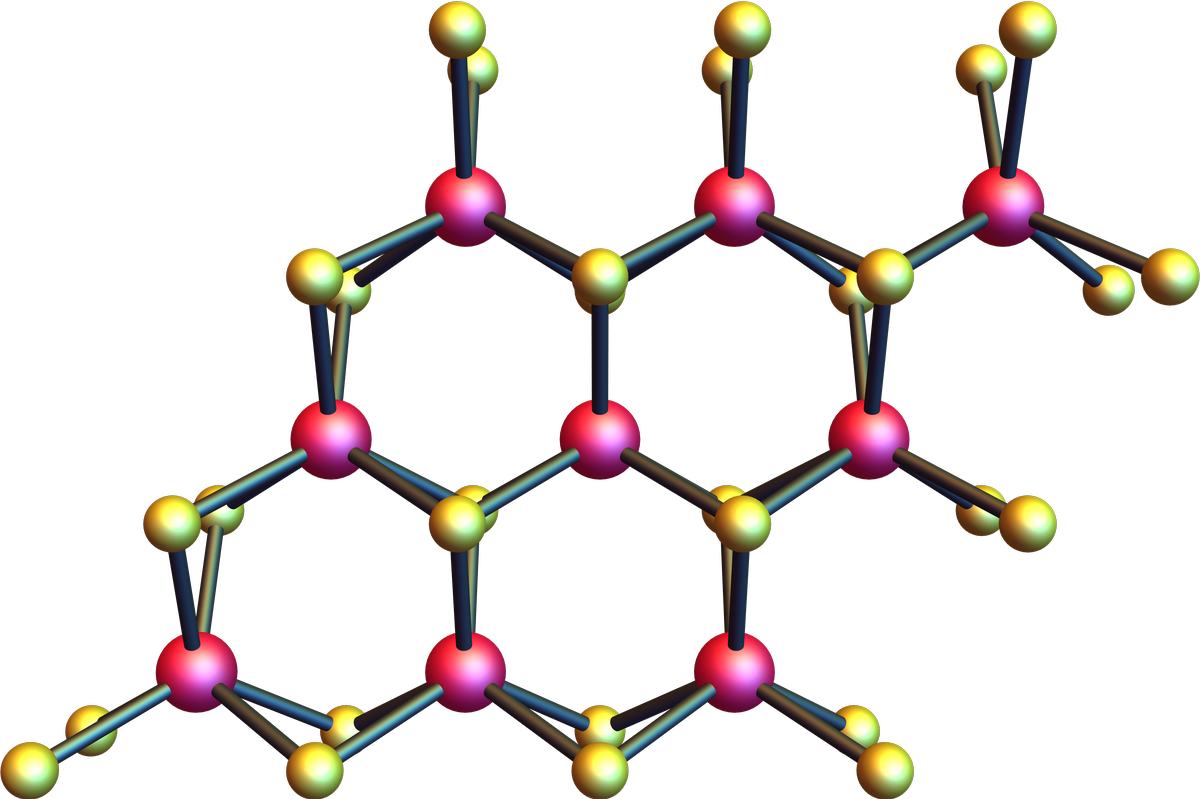
\includegraphics[width=0.7\textwidth]{figures/tmd-crystal-top.png}
  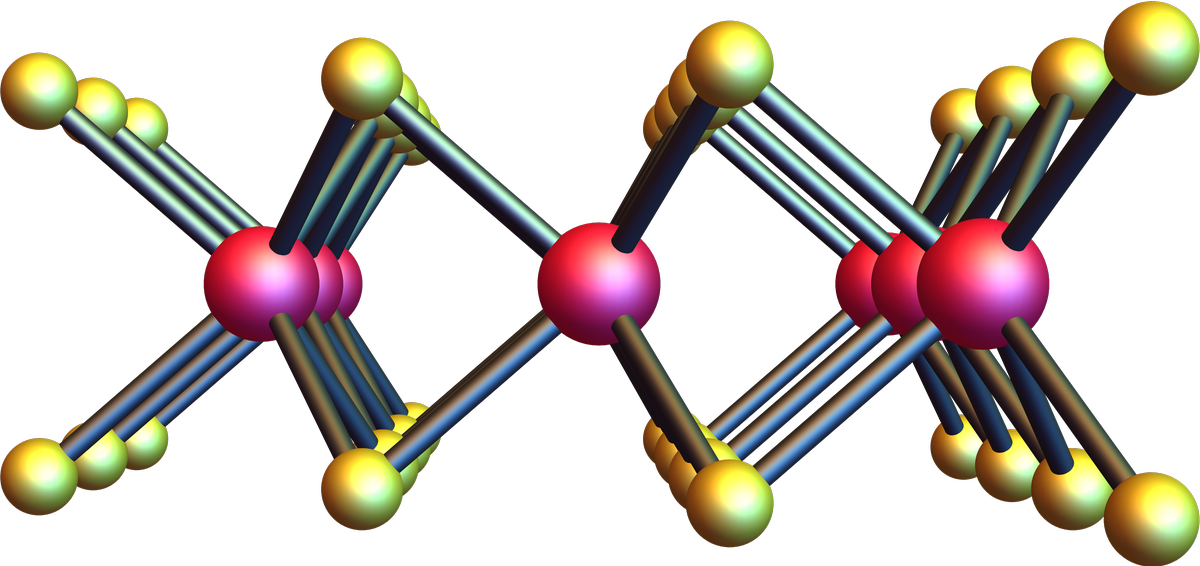
\includegraphics[width=0.7\textwidth]{figures/tmd-crystal-side.png}
  \caption{%
    Top and side views of the crystal structure of monolayer \ce{MoS2}.
  }\label{fig:tmd-crystal}
\end{figure}
